%\chapter*{Неделя 2}
\protect\thispagestyle{fancy}
\section{}
Даны два сигнала, представленные в виде линейной комбинации двух косинусоид:

\begin{align*}
x_1[k] = \cos( \pi k / 4)  + \cos(17 \pi k / 64),\\
x_2[k] = \cos( \pi k / 4)  + \cos(21 \pi k / 64).
\end{align*}

Вычисляется спектральная оценка каждого из этих сигналов с помощью $64$-точечного ДПФ  и $64$-точечного прямоугольного окна.
Определить, будут ли различимы спектральные максимумы в каждом из двух случаев.

\begin{align*}
x_1[k] &= \cos( \pi k / 4)  + \cos(17 \pi k / 64) = \cos( 8\cdot 2\pi k / 64)  + \cos(8.5 \cdot 2 \pi k / 64).\\
\mathcal{X}_1(\nu) &= \dfrac{1}{2}\left[\mathcal{W}_{\mathcal{D}}\left(\nu-\dfrac{8}{64}\right) +
\mathcal{W}_{\mathcal{D}}\left(\nu+\dfrac{8}{64}\right) +
\mathcal{W}_{\mathcal{D}}\left(\nu-\dfrac{8.5}{64}\right) +
\mathcal{W}_{\mathcal{D}}\left(\nu+\dfrac{8.5}{64}\right)\right]^{\footnotemark}.
\end{align*}
\footnotetext{$\Capit{W}_{\Capit{D}}(\nu) = \dfrac{\sin (N \pi \nu)}{\sin(\pi \nu)}e^{-j(N-1)\pi \nu}$ -- ДВПФ прямоугольного окна (окна Дирихле) из $N=64$ отсчётов.}

Расстояние между относительными частотами косинусоид $\Delta \nu = \frac{8.5-8}{64} = \frac{0.5}{64}$, то есть справедливо, что $\Delta \nu < \frac{0.89}{64} = \Delta \nu_{-3\text{dB}}$. В этом случае можно сделать вывод о том, что спектральные максимумы в ДПФ не будут различимы (сольются в один максимум).


\begin{align*}
x_2[k] &= \cos( \pi k / 4)  + \cos(21 \pi k / 64) = \cos(2\cdot 8\pi k / 64)  + \cos(10.5 \cdot 2 \pi k / 64).\\
\mathcal{X}_2(\nu) &= \dfrac{1}{2}\left[\mathcal{W}_{\mathcal{D}}\left(\nu-\dfrac{8}{64}\right) +
\mathcal{W}_{\mathcal{D}}\left(\nu+\dfrac{8}{64}\right) +
\mathcal{W}_{\mathcal{D}}\left(\nu-\dfrac{10.5}{64}\right) +
\mathcal{W}_{\mathcal{D}}\left(\nu+\dfrac{10.5}{64}\right)\right].
\end{align*}

Расстояние между относительными частотами косинусоид $\Delta \nu = \frac{10.5-8}{64} = \frac{2.5}{64}$, что превышает ширину главного лепестка окна на нулевом уровне $\Delta \nu_0 = \left(\frac{2}{64}\right)$. С учётом того, что абсолютные значения амплитуд максимумов совпадают, можно сделать вывод о том, что спектральные максимумы будут различимы как в ДВПФ, так и в ДПФ.

\begin{figure}[!h]
	\centering
	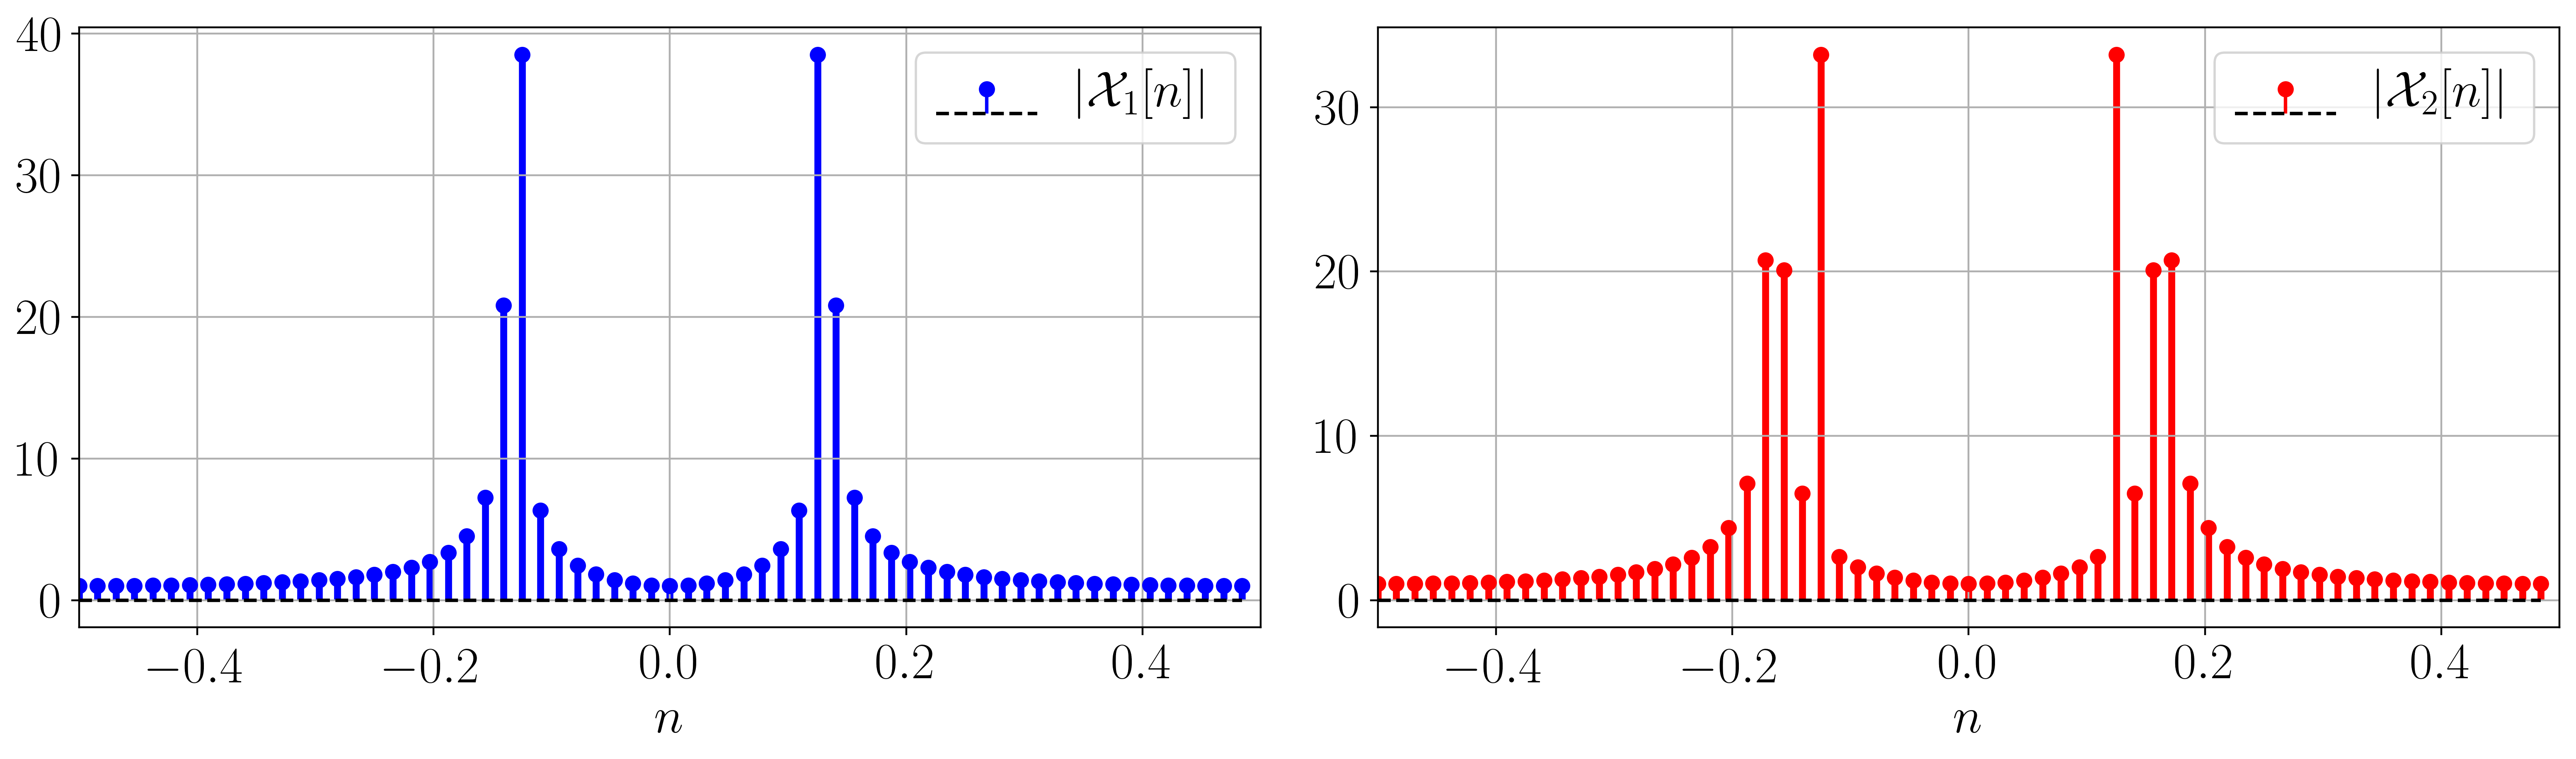
\includegraphics[width=1.\columnwidth]{pics/spring/2/2-1.png}
	%\caption{.}
	\label{fig:2-1}
\end{figure}



\newpage
\section{}
Пусть известно, что обрабатываемая последовательность имеет вид
\begin{equation*}
x[k] = \sum \limits_{m=0}^{M} \mathcal{A}_m \cos\left(2\pi\frac{m}{N}k + \varphi_m \right),\quad k = 0, 1, \ldots, N-1,
\end{equation*}

где $\mathcal{A}_m$ и $\varphi_m$ -- неизвестные заранее амплитуды и фазы гармонических составляющих;
$m$ -- неизвестные заранее целые числа, определяющие нормированные частоты $\nu_m = m/N$ гармонических составляющих, которые совпадают с бинами ДПФ.

Выразите неизвестные амплитуды и фазы через отсчёты ДПФ данной последовательности.

\begin{align*}
\mathcal{X}[n] &= \sum \limits_{k=0}^{N-1}x[k]e^{-j2\pi\frac{nk}{N}} = 
\sum \limits_{k=0}^{N-1} \left(\sum \limits_{m=0}^{M} \mathcal{A}_m \cos\left(2\pi\frac{m}{N}k + \varphi_m \right)\right) e^{-j2\pi\frac{nk}{N}} = \\
&= \dfrac{1}{2} \sum \limits_{m=0}^{M} \mathcal{A}_m
\sum \limits_{k=0}^{N-1} \left( e^{j(2\pi\frac{m}{N}k + \varphi_m)} + e^{-j(2\pi\frac{m}{N}k + \varphi_m)} \right) e^{-j2\pi\frac{nk}{N}} = \\
&= \dfrac{1}{2} \sum \limits_{m=0}^{M} \mathcal{A}_m \left( 
\sum \limits_{k=0}^{N-1}  e^{j(2\pi\frac{m-n}{N}k + \varphi_m)}
+  \sum \limits_{k=0}^{N-1}  e^{-j(2\pi\frac{m+n}{N}k + \varphi_m)}
\right) = \\
&= \dfrac{1}{2} \sum \limits_{m=0}^{M} \mathcal{A}_m \left( 
e^{+j\varphi_m}\sum \limits_{k=0}^{N-1}  e^{j2\pi\frac{m-n}{N}k}
+  e^{-j\varphi_m}\sum \limits_{k=0}^{N-1}  e^{j2\pi\frac{N-(m+n)}{N}k}
\right) = \\
&= \dfrac{N}{2} \sum \limits_{m=0}^{M} \mathcal{A}_m \left( 
e^{+j\varphi_m}\delta_{m, n}
+  e^{-j\varphi_m}\delta_{m, N - n}
\right) = \dfrac{N}{2} \left(\mathcal{A}_ne^{+j\varphi_n} + \mathcal{A}_{N-n}e^{-j\varphi_{N-n}}\right).
\end{align*}

Если $M \leq \lceil N/2 \rceil - 1$, то система уравнений будет однозначно и легко разрешима относительно неизвестных $\mathcal{A}_m$ и $\varphi_m$:

\begin{equation*}
\mathcal{A}_{m} = \dfrac{2}{N}|\mathcal{X}[m]|, \quad \varphi_m = \arg\{X[m]\}, \quad m=0, \ldots, M \leq \lceil N/2 \rceil - 1.
\end{equation*}

\section{}
Предположим, что нужно вычислить спектральную оценку дискретного сигнала с помощью ДВПФ и окна. При этом необходимо добиться разрешения не менее $\Delta \nu = 0.0075$, а длина окна фиксирована и равна $N = 256$. 

Используя данные из таблицы приложения к лекции, определить, какие из следующих окон гарантированно позволяют выполнить поставленную задачу:
а) прямоугольное,	б) Бартлета,	в) Ханна,\\	г) Хэмминга,	д) Блэкмана.

Заметим, что $\Delta \nu = 0.0075 = \frac{1.92}{N}$. Спектральные компоненты будут гарантировано различимы, если $\Delta \nu = \frac{1.92}{N} \geq \Delta \nu_{-6\text{dB}}$. Исходя из этого условия, заключаем, что для задачи подходят: 
а) прямоугольное окно $\left(\Delta \nu_{-6\text{dB}} = \frac{1.2}{N}\right)$,
б) окно Бартлета $\left(\Delta \nu_{-6\text{dB}} = \frac{1.78}{N}\right)$, 
г) окно Хэмминга $\left(\Delta \nu_{-6\text{dB}} = \frac{1.82}{N}\right)$.
